
\begin{figure}[hp]
%
\subcaptionbox{\label{fig:ecr-pair-ptci-hists-base}}
{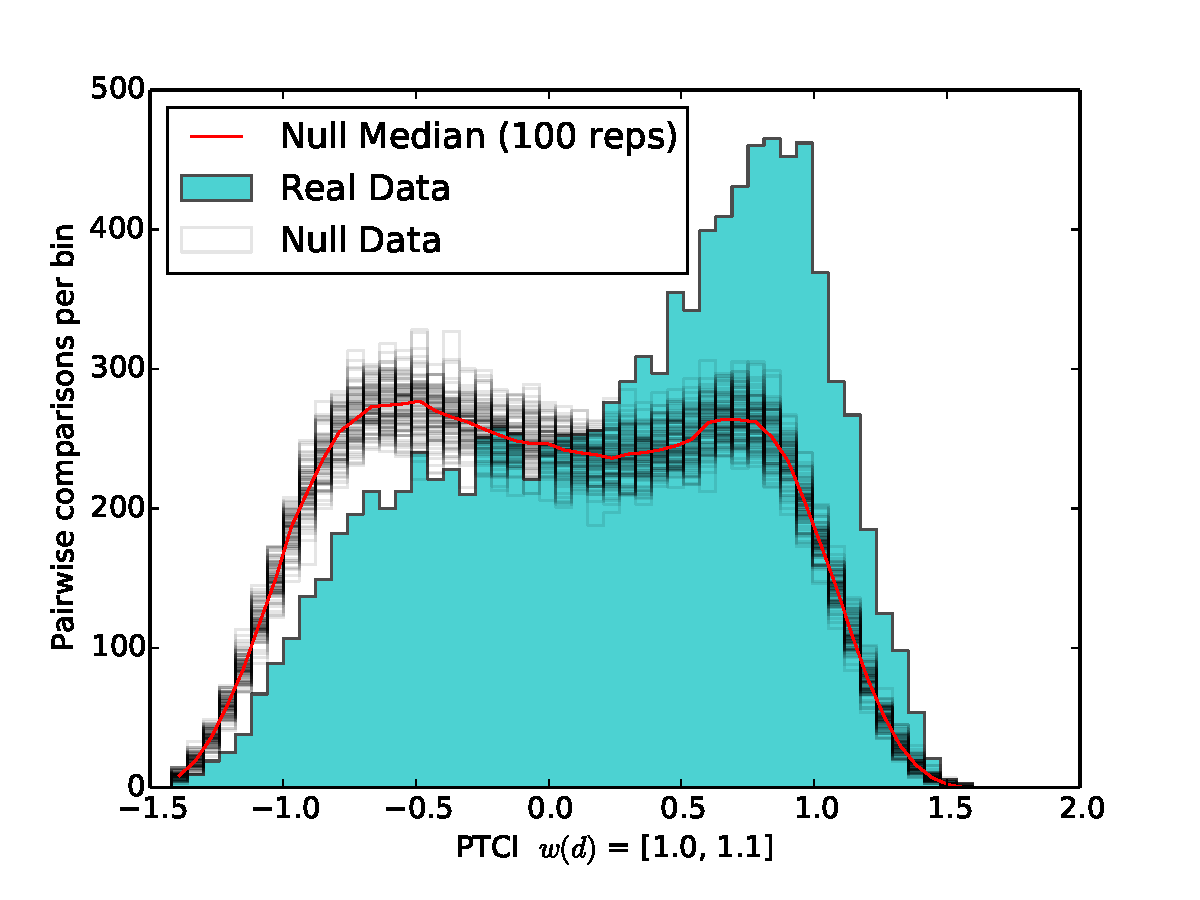
\includegraphics[width=.5\linewidth]{figures/figs/ecr_team_ptci_20130918_orthodb7/pairwise_ptci_hist.pdf}}
% 
\subcaptionbox{\label{fig:ecr-pair-ptci-hists-rcum-hist}}
{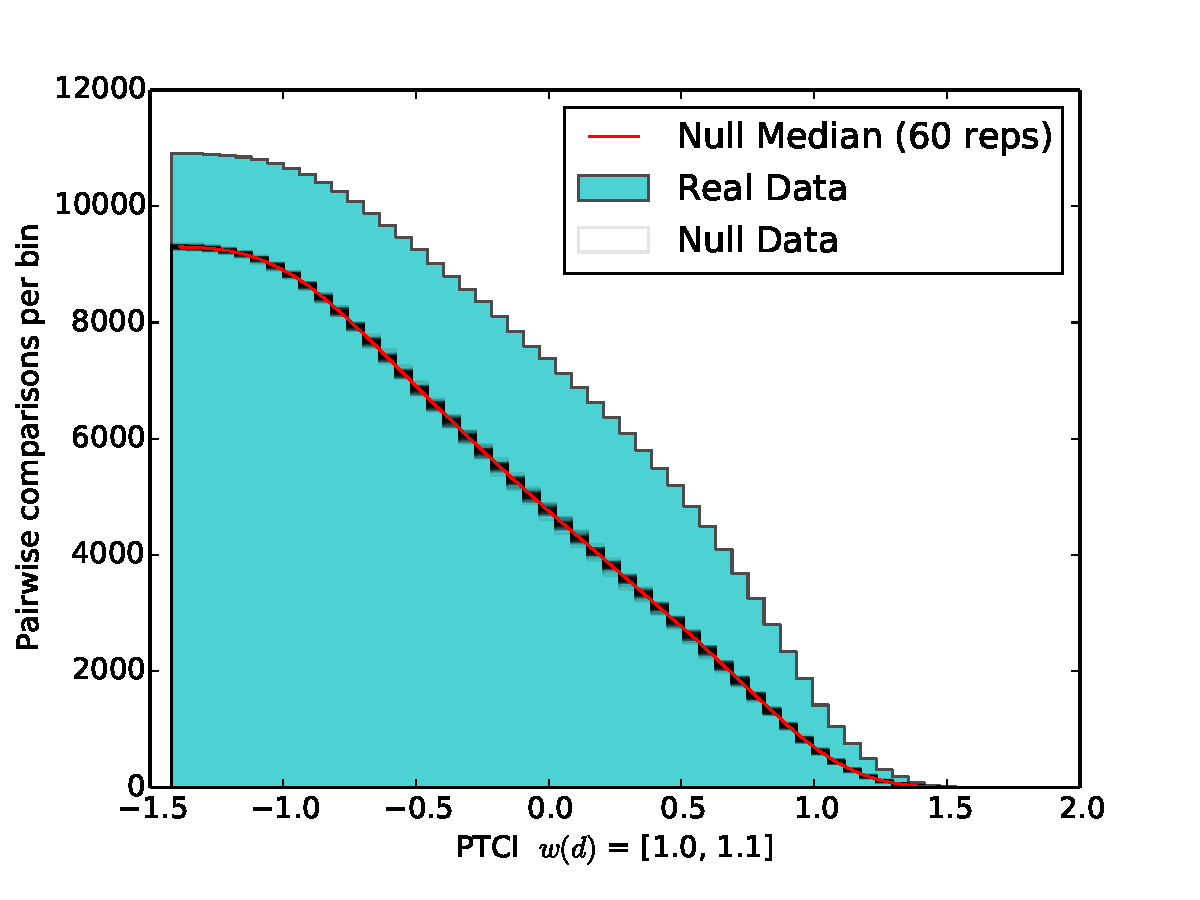
\includegraphics[width=.5\linewidth]{figures/figs/ecr_team_ptci_20130918_orthodb7/pairwise_ptci_cum_hist.pdf}}
% 
\subcaptionbox{\label{fig:ecr-pair-ptci-hists-fdr}}
{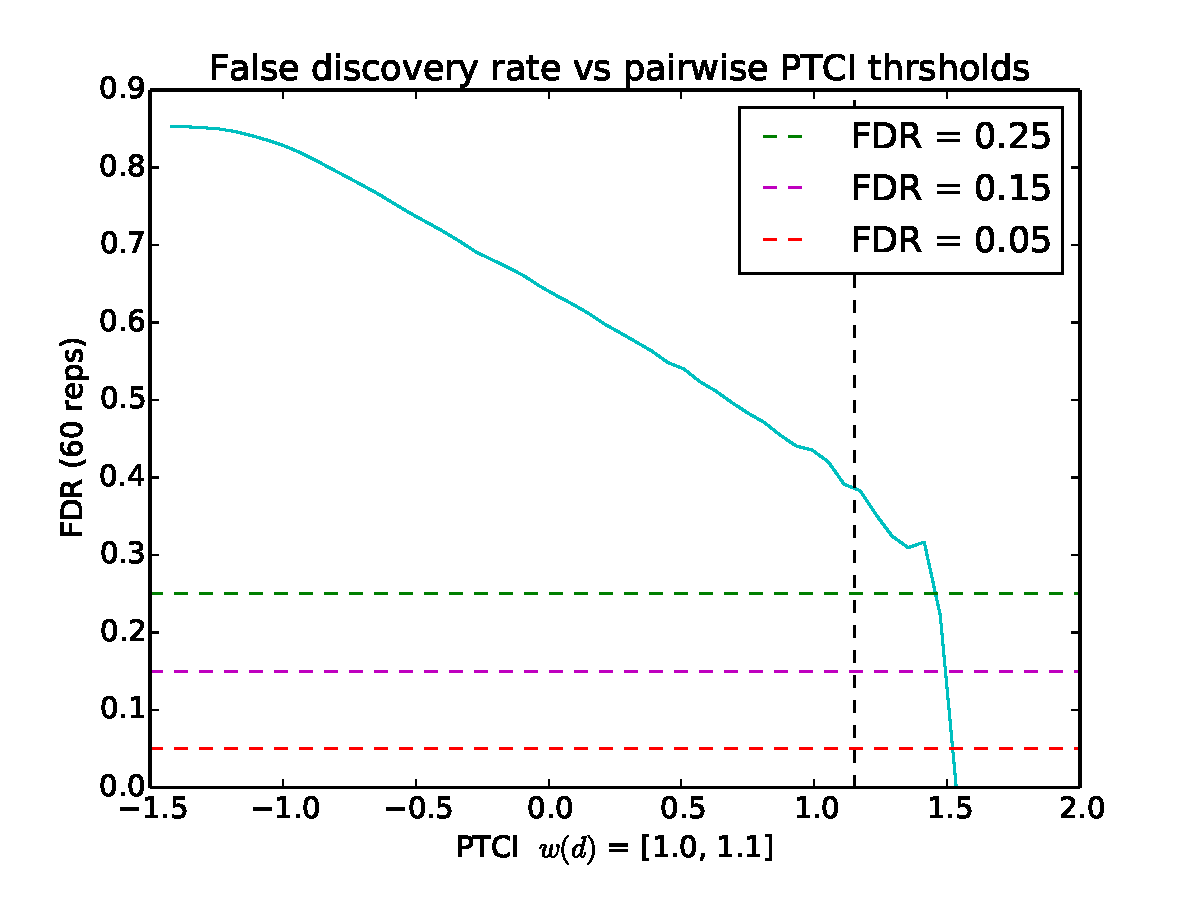
\includegraphics[width=.5\linewidth]{figures/figs/ecr_team_ptci_20130918_orthodb7/pairwise_ptci_fdr.pdf}}
% 
% 
\caption[Pairwise 20E-PTCI results]{\sf \textbf{Pairwise PTCI results for the \gls{20E}-\gls{TFBS} group}:\\
\textbf{(A)} Histogram of mean PTCI results vs null distributions.
\textbf{(B)} Reverse Cumulative histogram of mean PTCI results vs null distributions.
\textbf{(C)} False discovery rate vs PTCI threshold.}
\label{fig:ecr-pair-ptci-hists}
\end{figure}